\section{Metodología}

Durante la historia del desarrollo de software han surgido muchas metodologías de desarrollo ágil buscando facilitar este y asegurar su cumplimiento. Una de las metodologías de desarrollo más utilizadas es SCRUM. SCRUM fue presentado por primera vez en el artículo ``The new new Product development game'' \cite{takeuchi1986new}. Aunque inicialmente SCRUM está pensado para grupos de trabajo, en este caso será útil de aplicar ciertas partes de la metodología.

La metodología divide los actores en tres tipos de personas: Desarrolladores, Product Owner y Scrum Master \cite{schwaber2011scrum}. En este caso concreto, la metodología se planificó de forma que la tutora hiciese el rol de Product Owner asegurando que el producto llegue a buen término y que cumpla con los requisitos necesarios. Por otra parte, el alumno desarrollaría los roles de desarrollador y Scrum master. Aquí se busca ser capaz de hacerse cargo tanto del desarrollo, planear cada sprint, adaptar el plan a realizar para cada día de desarrollo, garantizar que la aplicación de SCRUM es la correcta, eliminar impedimentos del desarrollo entre otras funciones. 

Los sprints de desarrollo se fijaron en una duración de dos semanas cada uno, comenzando el día 1 de abril. En el primer día de cada sprint se realizaba la planificación de este, buscando las tareas a realizar en ese sprint en función del tiempo, y como se distribuye el trabajo en base a la carga de esas semana. Al ser un proyecto paralelo a otros, es decir, no se tenía un pleno tiempo de trabajo durante el sprint, estos se planificaban en base a la carga de trabajo externa de esa quincena. Cada día dedicado al proyecto, se planificaba las tareas a realizar ese mismo día. 

Cada día de finalización de los sprints, se realizaba una reunión de aproximadamente 30 minutos con la Product Owner buscando mejorar y corregir lo realizado durante el desarrollo. Estas reuniones normalmente aumentaban el trabajo a realizar para los siguientes sprints.

Aplicando esto, se llegó a un proceso iterativo donde cada iteración de desarrollo correspondía a un sprint. Previo a esto, se realizaron las reuniones con los clientes, para recabar toda la información necesaria y recoger los requisitos y objetivos según lo acordado. El flujo de trabajo quedaría finalmente como el indicado en la Figura \ref{fig:modelo_de_proceso}.

\begin{figure}[H]
    \centering
    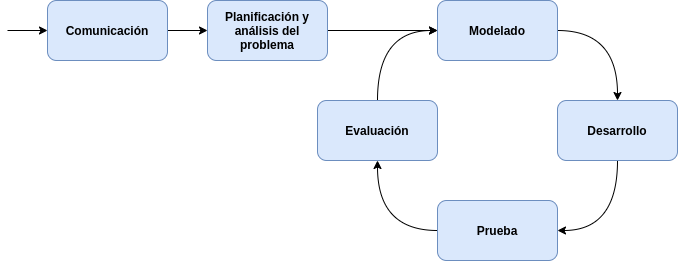
\includegraphics[width=\textwidth]{diseno/modelo_de_proceso.png}
    \caption{Modelo de proceso del proyecto}
    \label{fig:modelo_de_proceso}
\end{figure}

\section{Temporización}

Una vez decidida la metodología a aplicar, había que buscar una forma de planificar las tareas a realizar en el tiempo. Uno de los creadores de Scrum habla de como en el desarrollo de software ``generalmente el 80\% del valor de un producto de software reside en el 20\% de sus funcionalidades''\cite{sutherland-2014}. Bajo esta premisa, buscando garantizar el desarrollo de un producto completo, se ordenaron las funcionalidades en base a prioridades, garantizando de que en caso de que el producto no llegase a entregase de forma completa, se pudiese entregar una parte funcional de este.

Partiendo de lo comentado en reuniones con los clientes y de los requisitos establecidos, las partes o tareas del desarrollo se organizaron tal que así: 

\begin{itemize}
    \item Prioridad de nivel 4
    \begin{itemize}
        \item Sistemas de autenticación y de gestión de usuarios.
        \item Gestión de datos de personas sin contemplar relaciones entre ellos ni altas y bajas.
        \item Gestión de documentos asociados a las personas
        \item Gestión de datos de casas y habitaciones junto con sus residentes.
        \item Gestión de actividades y asistentes a estas sin puntuaciones.
    \end{itemize}
    \item Prioridad de nivel 3
    \begin{itemize}
        \item Uso de fotografías en personas, actividades y alojamientos.
        \item Gestión de altas y bajas de los residentes.
        \item Puntuaciones en los asistentes a las actividades.
        \item Gestión de citas asociadas a personas.
    \end{itemize}
    \item Prioridad de nivel 2
    \begin{itemize}
        \item Ranking de usuarios.
        \item Estadísticas.
        \item Búsqueda de personas por parámetros.
        \item Exportación de datos.
    \end{itemize}
    \item Prioridad de nivel 1
    \begin{itemize}
        \item Módulo de cámara insertado en la aplicación.
        \item Notificaciones de citas. 
    \end{itemize}
\end{itemize}

Estas características, algunas con más trabajo que otras, han sido ordenadas de forma que si se desarrollan las características siguiendo la prioridad establecida se podrá asegurar la entrega final de un producto válido.

\section{Seguimiento del desarrollo}

Como se ha indicado antes, cada sprint tenía una duración de 2 semanas. Para estas dos semanas se seleccionaban unas tareas a realizar a principio de la semana y al final de esta eran comentadas y revisadas por el Product Owner. Debido a que el desarrollo del proyecto no ocupaba el 100\% del tiempo de los integrantes, es posible que no todas las sesiones tuviesen o buscasen la misma carga de trabajo. Las sesiones fueron las siguientes:

\subsection{Inicio del desarrollo}

\textbf{Fecha de la sesión}: 1 de Abril de 2021

Durante la sesión se establecieron los objetivos a intentar completar en el primer sprint del proyecto. En este se establecieron los siguientes objetivos:

\begin{itemize}
    \item Diseño de la estructura de la base de datos y como se almacenan y relacionan los datos.
    \item Diseño del sistema de autenticación y gestión de roles.
    \item Implementación del sistema de autenticación en el backend.
    \item Implementación del inicio de sesión y gestión de usuarios.
\end{itemize}

\subsection{Revisión del primer sprint y preparación del segundo}

\textbf{Fecha de la sesión}: 15 de Abril de 2021

Esta fue la primera reunión de desarrollo con el Product Owner. Aquí se presentó lo realizado hasta el momento, y se debatió sobre otras cuestiones. En forma de resumen, se realizó lo siguiente:

\begin{itemize}
    \item Se propusieron cambios en como se relacionaban algunos de los datos.
    \item Se pregunto por el diseño de la arquitectura y como esta iba a ser
    \item Se mostró lo implementado hasta el momento, tanto lo referente al backend como al inicio de sesión en la aplicación. 
\end{itemize}

Tras esta reunión, se dedico tiempo a decidir las tareas a realizar en la sesión posterior:

\begin{itemize}
    \item Diseño en la arquitectura del sistema.
    \item Diseño de un diagrama de clases conceptual con el objetivo de clarificar las relaciones
    \item Corrección de los problemas de la iteración anterior (relaciones entre datos).
    \item Implementación de la base de datos en base al diseño realizado.
    \item Finalización de la gestión de usuarios, sin tener en cuenta su asociación a personas, parte todavía no implementada en el sistema.
\end{itemize}

\subsection{Revisión del segundo sprint y preparación del tercero}

\textbf{Fecha de la sesión}: 29 de Abril de 2021

Al final de la segunda sesión de desarrollo, de la misma manera, se tuvo una reunión con el Product Owner, en la cual sucedieron las siguientes cosas: 

\begin{itemize}
    \item Corrección sobre la representación de la arquitectura
    \item Validación y finalización de los diagramas referentes a la información y las relaciones entre sí.
    \item Muestra y validación de la gestión de usuarios desarrollada para la aplicación. 
\end{itemize}

Tras esta reunión, se dedico tiempo a decidir las tareas a realizar en la sesión posterior:

\begin{itemize}
    \item Corrección de la arquitectura presentada
    \item Desarrollo de la parte de gestión de personas tanto en la aplicación como en el backend.
\end{itemize}

\subsection{Revisión del tercer sprint y preparación del cuarto}

\textbf{Fecha de la sesión}: 13 de Mayo de 2021

Al final de la tercera sesión de desarrollo, de la misma manera, se tuvo una reunión con el Product Owner, en la cual sucedieron las siguientes cosas: 

\begin{itemize}
    \item Validación de la arquitectura
    \item Muestra del desarrollo de funcionalidades en el ámbito de las personas:
    \begin{itemize}
        \item Lista de personas por tipos.
        \item Obtención de la información de una persona en la aplicación.
        \item Eliminación de personas en la aplicación.
        \item Gestión de documentos asociados a las personas.
        \item Creación, edición y eliminación de personas en el backend.
    \end{itemize}
\end{itemize}

Tras esta reunión, se dedico tiempo a decidir las tareas a realizar en la sesión posterior:

\begin{itemize}
    \item Creación y edición de personas en la aplicación.
    \item Desarrollo de la gestión de alojamientos en la aplicación y backend.
    \item Desarrollo de la gestión de actividades en la aplicación y el backend.
\end{itemize}

\subsection{Revisión del cuarto sprint y preparación del quinto}

\textbf{Fecha de la sesión}: 27 de Mayo de 2021

Al final de la cuarta sesión de desarrollo, de la misma manera, se tuvo una reunión con el Product Owner, en la cual sucedieron las siguientes cosas: 

\begin{itemize}
    \item Muestra del funcionamiento de la edición y creación de personas en la aplicación.
    \item Muestra del funcionamiento de la gestión de alojamientos en la aplicación.
\end{itemize}

Tras esta reunión, partiendo de que algunas tareas no pudieron ser completadas en el sprint anterior, se dedico tiempo a decidir las tareas a realizar en la sesión posterior:

\begin{itemize}
    \item Desarrollo del apartado de actividades
    \item Gestión de fotografías en personas, actividades y alojamientos.
    \item Gestión de altas y bajas en las personas.
    \item Creación de citas asociadas a las personas.
\end{itemize}

\subsection{Revisión del quinto sprint y preparación del sexto}

\textbf{Fecha de la sesión}: 10 de Junio de 2021

Al final de la quinta sesión de desarrollo, de la misma manera, se tuvo una reunión con el Product Owner, en la cual sucedieron las siguientes cosas: 

\begin{itemize}
    \item Muestra del funcionamiento de la gestión de actividades en la aplicación.
    \item Muestra del uso de fotografías para los personas, actividades y alojamientos.
    \item Muestra del sistema de altas y bajas y como afectan a las personas del sistema.
\end{itemize}

Tras esta reunión, partiendo de que algunas tareas no pudieron ser completadas en el sprint anterior, como son las referentes a las citas asociadas, se dedico tiempo a decidir las tareas a realizar en la sesión posterior:

\begin{itemize}
    \item Desarrollo del sistema de citas y muestra de todas las citas en la aplicación.
    \item Búsqueda de personas en el backend.
    \item Desarrollo del sistema de estadísticas.
    \item Desarrollo del ranking en base a las puntuaciones de los usuarios.
    \item Exportación de datos 
    \item Sistemas de notificaciones de citas pasadas.
    \item Módulo de cámara insertado en la aplicación.
\end{itemize}

\subsection{Revisión del sexto sprint y preparación de la entrega}

\textbf{Fecha de la sesión}: 10 de Junio de 2021

Al final de la sexta sesión de desarrollo, de la misma manera, se tuvo una reunión con el Product Owner, en la cual sucedieron las siguientes cosas: 

\begin{itemize}
    \item Muestra del funcionamiento del sistema de citas.
    \item Muestra de la búsqueda de personas.
    \item Muestra del sistema de estadísticas.
    \item Muestra del sistema de puntuación y ranking de usuarios.
    \item Muestra de la exportación de datos.
\end{itemize}

Tras esta reunión, se concretaron y corrigieron ciertas cosas a preparar para la última entrega:

\begin{itemize}
    \item Desarrollo del módulo de cámara para añadir documentos.
    \item Revisión y finalización de la entrega.
\end{itemize}